%#####################################################################
% Author: Dr. Julien Nembrini, Manuel Mondal Simon Studer, Prof. Béat Hirsbrunner, 
% Created: 2015-03-23
% Modified: 2016-04-21,2019-02-11
% Description: latex template for project 1 report
%#####################################################################
\documentclass[11pt,a4paper]{report}

\usepackage[head=14pt,left=1in,right=1in, bottom=1in]{geometry} % to modify geometry
\usepackage[utf8]{inputenc}                           % to allow utf-8 encoding input e.g. ö é ä etc.
\usepackage[english]{babel}			                  % 
%\usepackage[frenchb]{babel}			              % PLEASE UNCOMMENT TO FIT THE LANGUAGE YOU USE
%\usepackage[german]{babel}			                  % 
\usepackage[pdftex]{graphicx}                         % to include graphics
\usepackage{amsmath}                                  % for maths functions
\usepackage{amsfonts}                                 % for maths fonts
\usepackage{amssymb}                                  % for maths symbols
\usepackage[hidelinks]{hyperref}                      % to allow urls and inner references
\usepackage{titling}                                  % for fancy titles
\usepackage{caption}                                  % for fancy captions
\usepackage{listings}                                 % to include listings
\usepackage{color}                                    % for custom colors
\usepackage{pgf}                                      % for special drawings 
\usepackage{tikz}                                     % for special drawings 

\usepackage{blindtext}                                % for placeholder text

\usetikzlibrary{arrows,automata}                      % for FSM diagrams

%################### Preamble Start #####################################


%%%%%%%%%%%%%%%%%%%%
% move title to top of page
\setlength{\droptitle}{-10em}


%%%%%%%%%%%%%%%%%%%%
% setup page
%\sloppy
%\pagenumbering{roman}
%\pagestyle{plain}
%\pagenumbering{arabic}
%\pagestyle{headings}

% header and footer
\usepackage{lastpage}
\usepackage{fancyhdr}
\pagestyle{fancy}
\fancyfoot[R]{\thepage/\pageref{LastPage}}
\fancyfoot[C]{}
\fancyfoot[L]{\footnotesize\emailurl{\myemail}}
\fancyhead[L]{\thetitle}
\fancyhead[R]{\theauthor}


% remove additional space between tables and their captions
%\captionsetup[table]{skip=0pt}


\graphicspath{{figures/}}


%%%%%%%%%%%%%%%%%%%%
% Listings

\definecolor{codegreen}{rgb}{0,0.6,0}
\definecolor{codegray}{rgb}{0.5,0.5,0.5}
\definecolor{codepurple}{rgb}{0.58,0,0.82}
\definecolor{backcolour}{rgb}{0.99,0.99,0.97}

\lstdefinestyle{customc}{
  belowcaptionskip=1\baselineskip,
  breaklines=true,
  frame=single, 
  tabsize=4, 
  numbers=left,
  numberstyle=\tiny\color{codegray},
  stepnumber=2,
  xleftmargin=\parindent,
  language=C,
  showstringspaces=false,
  basicstyle=\tiny\ttfamily,
  %basicstyle=\tiny,
  backgroundcolor=\color{backcolour},   
  commentstyle=\color{codegreen},
  keywordstyle=\color{codepurple},
  stringstyle=\color{blue},
  identifierstyle=\color{black},
}

\lstset{escapechar=@,style=customc} % set default language

%\lstset{language=C} 

%%%%%%%%%%%%%%%%%%%%
% TODO box

\newcommand{\todo}[1]{\par \noindent
\begin{minipage}[c]{0.95 \textwidth}
\textit{#1} \end{minipage}\par}

\newcommand{\emailurl}[1]{\href{mailto:#1}{#1}}
\newcommand{\email}[1]{\gdef\myemail{#1}}
\newcommand{\address}[1]{\gdef\myaddress{#1}}
%\newcommand{\keywords}[1]{\begin{center}{\bfseries Keywords:} #1\end{center}}
\newcommand{\keywords}[1]{\vskip \baselineskip \noindent{\bfseries Keywords:} #1 \vskip \baselineskip \par}

\renewcommand\maketitle{
\begin{center}%
    {\huge \thetitle \vskip \baselineskip \par}%
    {\large \theauthor \vskip \baselineskip \par}%
\myaddress
\emailurl{\myemail}
\end{center}
}

%################### Preamble Stop #####################################


% title setup
\title{Robotics Project I}
\date{\today}
\author{Firstname \textsc{Lastname}, Group 0}
\address{IN.2022 Robotics 2019, BSc Course, 2nd Sem.\\
University of Fribourg \\}
\email{firstname.lastname@unifr.ch}
	

\begin{document}
%################### Report Start #####################################


\maketitle
\thispagestyle{empty}



\begin{abstract}
\noindent Brief description of the content (5-10 lines). Helps people decide whether the report is relevant for them or not. Usually written at the end.

\keywords{add, keywords, for, indexing}


The use of \LaTeX\ is mandatory for the Project I report. Apart from the examples in the appendix below, this template may not be modified. A good introduction to scientific writing is given by \cite{Writing} 

\end{abstract}

\tableofcontents

%\newpage


\chapter{Introduction}
Objectives of this project,  and brief description of the structure of the report.



\chapter{Sensors}
Chapter about the sensors that will be used during Project I


\section{Proximity infra-red sensors}
Description of the sensors and graphs of measurements

\section{Infra-red ground sensor}
Description of the sensor and graphs of measurements

\section{Camera}
Description of the camera and graphs of measurements



\chapter{Behaviours}
Chapter about the behaviours that will be implemented for the assignments

\section{Braitenberg vehicle}
Description of the braitenberg behaviours

\subsection{LOVER}
\subsection{EXPLORER}


\section{Line-following}
Description of the line following behaviour using a braitenberg (reactive) controller

\section{Wall-following}
Description of the wall-following behaviour using a PID controller (including a description of the PID in general)

\section{Color recognition}
Description of the color recognition behaviour

\section{Multi-robot coordination}
Description of the Multi-robot coordination using communication between robots

\chapter{Conclusion}
Synthesis of the report and outlook for further work.



%------------------- Bibliography Start -------------------------------
\begin{thebibliography}{20}
\bibitem{Writing}
Justin Zobel.											% author
\textit{Writing for Computer Science}, 2nd edition.		% title (italics), edition
Springer-Verlag, London, 2004, 275 pages.				% editor, date, other info

% book source
\bibitem{Braitenberg} % cited with '\cite{Braitenberg}'
Valentino Braitenberg.									% author (Firstname Lastname, Firstname2 Lastname2, ...)
\textit{Vehicles: Experiments in Synthetic Psychology}.	% title (italics)
MIT Press, 1986.										% editor, date

% web source
\bibitem{WebotsEpuck} % cited with '\cite{WebotsEpuck}'
														% author (sometimes not available)
\textit{Webots Reference Manual}.					    % title (italics)
\url{https://www.cyberbotics.com/reference.pdf}			% url
version 2019a											% version
Last visited: 11.02.2019.   							% date
\end{thebibliography}
%------------------- Bibliography End -------------------------------


%################### Report End #####################################
%################### Appendix Start #####################################

\renewcommand{\thesubsection}{\Alph{section}.\arabic{subsection}}

\newcommand{\appendi}[1]{%
  \refstepcounter{section}%
  \section*{Appendix \Alph{section} #1}%
  \addcontentsline{toc}{section}{Appendix \Alph{section} #1}%
}

\chapter*{Appendix}
\addcontentsline{toc}{chapter}{Appendix}%


\appendi{Experimental Results}
Place to list the gathered data.

\appendi{Source Code} \label{app:sourceCode}
Place to list source code.

\subsection{IR sensors calibration procedure} \label{app:calib} % referenced with '\ref{app:calib}'
The code below shows the IR sensor calibration procedure.
\lstinputlisting[firstline=46, lastline=66]{code/S03_State_Machine_Sol.c}


%------------------- TODO: Remove Examples Start -------------------------------
\appendi{\LaTeX\ Examples} % only for demonstration, remove this section
This section shows some common uses of \LaTeX\ features.
\subsection{Images}
Example of how to include an image can be seen in Figure \ref{fig:graphicfile}. All figures must be referenced somewhere in the report.
\begin{figure}[ht!]
\begin{center}
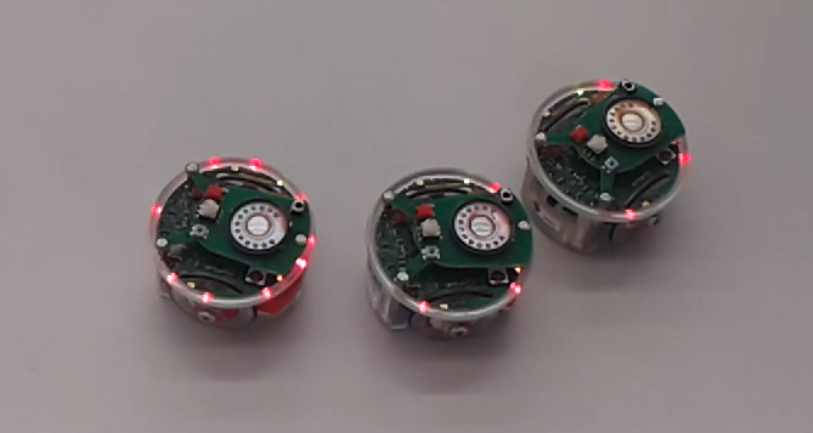
\includegraphics[width=7cm]{chain}
\caption{Including an image.}
\label{fig:graphicfile} % no file ending
\end{center}
\end{figure}

\subsection{Tables}
Example of how to include a table can be seen in Figure \ref{fig:someTable}. All figures must be referenced somewhere in the report.
\begin{figure}[ht!]
\begin{center}
\begin{tabular}{|c|c|}
\hline
\textbf{Title 1} & \textbf{Title 2} \\
\hline
item 11	&	item 12	\\
\hline
item 21	&	item 22	\\
\hline
\end{tabular}
\end{center}
\caption{Table with caption.}
\label{fig:someTable}
\end{figure}

\subsection{Listings}
Example of how to include listing can be seen in Figure \ref{fig:listing1} and Figure \ref{fig:listing2}. All figures must be referenced somewhere in the report.
\begin{figure}[ht!]
\lstinputlisting[firstline=46, lastline=66]{code/S03_State_Machine_Sol.c}
\caption{Listing included from file.}
\label{fig:listing1}
\end{figure}
\begin{figure}[ht!]
\begin{lstlisting}
// constrain speed to +/- MAX_SPEED
double bounded_speed(double speed) { 
  if (speed > MAX_SPEED) return MAX_SPEED;
  else if (speed < -MAX_SPEED) return -MAX_SPEED;
  else return speed;
}
\end{lstlisting}
\caption{Listing within \LaTeX.}
\label{fig:listing2}
\end{figure}

\subsection{Font Style and Text Size}
The font style may be modified: \textbf{bold}, \textit{italic}, \emph{Emphasis}, \textsc{Capitals}, \verb|verbatim|, etc.\\
The text size can be changed: \tiny tiny, \small small, \large large, \huge huge, \normalsize etc.

\subsection{Enumerations and Other Lists}
Enumerations are easy, there is the
\texttt{enumerate} environment:
%
\begin{enumerate}
  \item First item
  \item Second item
  \item Third item
\end{enumerate}

\noindent For lists, there is the
\texttt{itemize} environment:
%
\begin{itemize}
  \item First item
  \item Second item
  \item Third item
\end{itemize}

\noindent For definitions lists, there is the \texttt{description} environment:
\begin{description}
\item[First term] -- Description of the first term
\item[Second term] -- Description of the second term
\end{description}

\subsection{Quotations and References}
Books and other documentation can be referenced as \cite{Braitenberg} and
websites as \cite{WebotsEpuck}.


\subsection{FSM diagram}

In Figure \ref{fig:fsm} is depicted a Finite State Automata diagram as presented in Lecture 02.

\begin{figure}[ht!]
\begin{center}
\begin{tikzpicture}[>=stealth,shorten >=1pt,auto,node distance=4cm]
  \node[initial,state] (l)      {locked};
  \node[state]         (ul) [right of=l]  {unlocked};

  \path[->] (l)  edge [loop above] node {push} (l)
                 edge [bend left]      node {coin} (ul)
            (ul) edge [bend left]      node {push} (l)
                 edge                  node {time=T} (l)
                 edge [loop above]     node {coin or time<T} (ul);

\end{tikzpicture}	
\end{center}
\caption{FSM diagram in \LaTeX.}
\label{fig:fsm}
\end{figure}


%------------------- TODO: Remove Examples End -------------------------------


%################### Appendix End #####################################
\end{document}
